\chapter{Evaluation der Zuverlässigkeit}
Nach der Erstellung eines Kubernetes-Clusters für eine Produktionsumgebung muss getestet werden, ob die Zuverlässigkeit im Vergleich zum aktuellen System, das mit Docker Compose deployed ist, gestiegen ist.
Dazu wird das Verhalten beider Systeme unter Last und bei Ausfällen in gleichen Szenarien getestet.
Damit soll entschieden werden, ob Kubernetes mit seinen Funktionen genügend Auswirkungen hat, um das aktuelle Docker-Compose-Deployment zu ersetzen, obwohl dieses für eine komplexere Verwaltung und einen höheren Ressourcenverbrauch sorgt. 
\section{Bewertungsgrundlagen und Metriken}
Die Zuverlässigkeit, die gemessen werden soll, kann in vier Oberkategorien aufgeteilt werden.

Die erste Kategorie ist die Verfügbarkeit. Dabei wird gemessen, wie gut der Service erreichbar ist. Das wird vor allem daran gemessen, ob der Service bei Ausfällen Request bearbeiten kann.
Es wird auch gemessen, wie lange ein Service bei einem Ausfall offline bleibt.
 
Die zweite Kategorie ist die Fehlertoleranz. Dabei soll gemessen werden, wie mit Fehlern bei Ausfällen und bei Last umgegangen wird.
Dabei wird vor allem die Error Rate gemessen, die während der Szenarien auftritt, sowie die Frage, ob es zu einem Neustart kommt.

Die dritte Kategorie ist die Stabilität. Dabei wird das Verhalten unter steigender Last getestet.
Dafür wird zueinen der CPU- und RAM-Verbrauch der Anwendung, aber auch vom gesamten Systems erfasst. Damit soll auch getestet werden, wie die Umgebung die Last skaliert.

Die vierte Kategorie ist die Wiederherstellbarkeit, also die Zeit, die benötigt wird, um den Service nach einem Ausfall wiederherzustellen.
Dabei wird die TTR (Time to Recovery) gemessen, also die Zeit, die ein System zum Wiederherstellen des Services braucht.

Eine Kategorie, die nur teilweise betrachtet wird, ist die Performance. Zwar beeinflussen sich Performance und Zuverlässigkeit gegenseitig, dennoch sind das zwei verschiedene Aspekte, die meist Hand in Hand gehen.
Dennoch werden die p95-Latenz und die durchschnittliche Response Time mitgemessen.

Mithilfe eines eigens erstellten Scoring-Verfahrens soll die Zuverlässigkeit bei jedem Test von 0 bis 100 bewertet werden.
Das Scoring beginnt mit einem Wert von 100 und nimmt ab, wenn die aufgenommenen Metriken auf eine eher schlechte Zuverlässigkeit hinweisen. Die Untergrenze bei jedem Scoring ist 0.
Dieses Scoring soll dabei helfen, die beiden Systeme besser vergleichen zu können. Je nachdem, was getestet wird, kann sich das Scoring unterscheiden.

Die Metriken sind normalisiert, damit beide Systeme besser verglichen werden können.
\section{Testaufbau und Testverfahren}
Um die Zuverlässigkeit zu testen, wurden beide Umgebungen unter vergleichbaren Bedingungen getestet. 
Dabei kamen verschiedene Testverfahren zum Einsatz, um die verschiedenen Kategorien der Zuverlässigkeit zu testen.
Dabei wurde sehr darauf geachtet, dass die Testverfahren einen fairen Vergleich ermöglichen.
Die Tests umfassten Loadtests und Chaostests mit jeweils eigenen Szenarien. 
Um reproduzierbare Ergebnisse zu erhalten, wurden die Durchführung der Tests sowie ihre Auswertung automatisiert.
Die folgenden Abschnitte beschreiben die Testumgebungen und -verfahren sowie deren Auswertung.

\subsection{Testumgebung}
Beide Umgebungen sollten mit der entsprechenden Hardware, auf der die Systeme betrieben werden, getestet werden.
Daher wurden weder das lokale Docker Compose noch der Kind-Cluster verwendet. 
Dies würde auch falsche Testdaten produzieren, da auf dem eigenen Rechner weitere Prozesse laufen als nur diese Umgebungen.
Zum anderen würden die Services im Dev-Modus laufen und Docker Compose würde der Traefik-Service fehlen. 
Der Kind-Cluster hat auch keine HA-Architektur und zusätzlich hat jeder Service nur einen Pod, um Last auf den lokalen Geräten zu sparen, da auch wenn Kind mit Docker drei Nodes simuliert, alle Nodes dennoch auf einer Hardware betrieben werden.

Daher werden die im Hochschulnetzwerk betriebenen Umgebungen genutzt. Bei Kubernetes wäre dies der k3s-Cluster.
Bei Docker Compose wurde allerdings die Staging-Umgebung genutzt, um den Betrieb in der Produktionsumgebung nicht zu stören.
Diese beiden Umgebungen unterscheiden sich jedoch nicht voneinander, wodurch die Ergebnisse nicht unterschiedlich ausfallen würden.

Um den Ressourcenverbrauch und die Container-Gesundheit in beiden Umgebungen messen zu können, wurden Grafana und Prometheus als Monitoring-Tools in beiden Umgebungen eingefügt.

Um in den Loadtests und Chaos-Tests Last zu erzeugen, wurde k6 verwendet. 
Mit k6 wurde nicht nur die Last erzeugt, sondern auch die Fehlerrate, die Antwortzeit sowie die Anzahl der Requests pro Sekunde gemessen.
Die Entscheidung, k6 als Loadtest-Tool zu verwenden, wurde getroffen, da sich mit k6 durch die skriptbasierte Erstellung von Testfällen und Testszenarien, diese sich flexibler definieren lassen und sich gut automatisieren lassen. 
Dadurch vereinfachten sich auch die Wiederholbarkeit und die Wiederverwendung von Tests.

Das Auslösen der Tests, die Produktion der Last sowie das Einsammeln der Testergebnisse wurden nicht auf den gleichen Umgebungen ausgeführt wie eine der Testumgebungen.
Dadurch sollte verhindert werden, dass während der Tests zusätzliche Lasten auf den Umgebungen entstehen, die die Testergebnisse verfälschen könnten.
Stattdessen wurden die Tests auf dem eigenen Rechner ausgeführt. Dieser diente als Client, der die Last an die Testumgebung verschickte.

Damit die Tests leicht reproduzierbar sind und jedes Mal gleich ausgeführt werden, wurden sie so erstellt, dass sie vollständig automatisiert durchgeführt werden können.
Der Ablauf der Automation ist wie folgt, zunächst wird sie mit der Information gestartet, welche Tests ausgeführt werden sollen. 
Nach dem Start verbindet sich die Automation über einen SSH-Tunnel mit dem Monitoring, bereitet die Testumgebung vor, indem beispielsweise die Testuser in der Datenbank erstellt werden und führt anschließend den Test aus.
Nach dem Test räumt die Automation die Testumgebung wieder auf, sodass sie sich wieder im Zustand vor dem Test befindet. Anschließend sammelt sie die Testdaten vom Monitoring ein und wertet diese zusammen mit den k6-Testdaten aus.
Dies wird für jeden angegebenen Test durchgeführt, bis alle dran gewesen sind.

Während der Tests war das Deployment gesperrt, damit alle Tests unter gleichen Bedingungen durchgeführt werden konnten.
Alle Tests wurden dreimal pro Umgebung ausgeführt, um sicherzustellen, dass keine einzelnen Testläufe die Umgebung unnötig verschlechtern.
\subsection{Loadtests}
Mit den Loadtests sollte primär das Verhalten der beiden Umgebungen unter Last, also ihre Stabilität, verglichen werden.
Gleichzeitig konnte die Fehlertoleranz unter Last beobachtet werden, indem die Fehlerrate betrachtet wurde.
Es wurden verschiedene Arten von Loadtests ausgeführt. Der kleinste ist der Smoke-Test, der in kurzer Zeit die kleinste Last produziert, die deutlich unter der Last liegt, die für den Normalbetrieb geplant ist.
Dabei begrenzt sich die Anzahl der virtuellen Nutzer meistens auf fünf.
Eine höhere Last ergibt sich bei dem Average-Load-Test und dem Stress-Test. Der Average-Load-Test testet die Last, die im geplanten Normalbetrieb auftreten soll.
Mit der IT und Herrn Boger wurde abgesprochen, dass die Anzahl der Nutzer im Normalbetrieb zunächst bei 100 liegt. Beim Average-Load-Test wird die Last zehn Minuten lang aufrechterhalten.
Beim Stress-Test ist die Last höher als im Normalbetrieb. Dies wurde mit 200 Nutzern umgesetzt, die die Last ungefähr gleich lang wie beim Average-Load-Test erzeugten.
Ein Spike-Test wurde ebenso durchgeführt. Dieser erzeugt eine kurze, plötzliche Lastspitze, wie sie z. B. beim Start eines Ticketverkaufs für ein großes Event, wie z. B. den Eurovision Song Contest, häufig auftritt.
Bei diesem Test wird in sehr kurzer Zeit extrem viel Last erzeugt, hier wären es 10 s. Im Test betrug diese 500 Nutzer. Allerdings wurde bei diesem Test eine kurze Warm-up- und Cooldownphase eingebaut, damit nicht nur alles abstürzt, wenn aus dem Leerlauf heraus eine solche Last passiert.
In dieser mindestens 1 Minute langen Phase nutzen 50 Nutzer die Anwendung. 
Zum Schluss wurden Breakingpoint-Tests ausgeführt, die über die Zeit linear immer mehr Last erzeugen, um das System an den Rand des Absturzes zu bringen.
Dabei stieg die Nutzerzahl innerhalb von 10 Minuten auf 400.

Die Testdateien selbst waren sehr generisch aufgebaut, um wiederverwendbar zu sein. Einstellungen zu den Tests, wie beispielsweise die Länge, wurden mit JSON geladen.
Im Setup und TearDown in K6 wurden Annotationen an Grafana verschickt, um den Start und das Ende der Loadtests zu markieren. Diese wurden verwendet, um die passenden Monitoring-Daten abzurufen.
In den Tests selbst wurden mehrere realistische Userflows durchgeführt, die durch einen Mapper passend zu einem virtuellen User zugeordnet wurden. 
Die Userflows wurden erstellt, indem diese nachgestellt wurden, während das Chrome DevTool die Aufrufe aufgenommen hat und sie so nah wie möglich als Userflow umgewandelt wurden.
Welche Userflows genutzt wurden und wie viele dieser prozentual über die virtuellen User vergeben wurden, war abhängig von den Szenarien.

Es gibt drei Szenarien. Im ersten Szenario gibt es nur einen UserFlow, in dem sich die virtuellen User in Codetask einloggen. Damit sollte speziell die Authentifizierung getestet werden.
Das Einloggen in den anderen Szenarien fällt damit weg, damit diese Szenarien getestet werden und nicht immer wieder die Authentifizierung.

Das zweite Szenario waren die Vorlesungen. Dieses Szenario sollte den Normalbetrieb nachahmen. Dabei gibt es zwei verschiedene Userflows für Studierende.
Einige Studierende durchlaufen die Vorlesungen und erfüllen die Aufgaben, während andere bei der Bearbeitung der Aufgaben unkonzentriert sind und zwischendurch durch die Website klicken.
Ein weiterer Userflow ist für die Lehrenden auf der Plattform vorgesehen. Sie überwachen Statistiken und verwenden die Editoren für Kurse und Aufgaben.
Der letzte Userflow simuliert einen sehr kleinen Anteil von Personen, die Codetask nur nebenbei geöffnet haben, während sie sich mit etwas anderem beschäftigen.

Das dritte Szenario sind die Klausuren, da dies der kritische Punkt bei Codetask ist, der zuverlässig funktionieren muss.
Zwei der User Flows richten sich komplett auf die Klausuren. Der eine richtet sich an die Studierenden, die an ihrer Klausur arbeiten, der andere an die Prüfenden, die die Klausur über Codetask überwachen.
Da Codetask flächendeckend benutzt werden soll, sind für die Klausuren auch die beiden UserFlows enthalten, in denen die Studierenden ihre Kurse bearbeiten und auch der Flow, in dem Personen Codetask im Leerlauf verwenden.

Es war geplant, die Quiztasks als Szenario zu testen, da diese als Testat benutzt werden sollten. Zum Zeitpunkt der Tests waren sie jedoch zu fehlerhaft, um sie richtig testen zu können.
\subsection{Chaos-Tests}
Die Chaos-Tests sollen das Verhalten der Umgebung bei Ausfällen testen.
Dabei wurde von K6 Last erzeugt. Dies entspricht 50 Studierenden, die über einen Zeitraum von 10 Minuten Aufgaben in Codetask bearbeiten.
Währenddessen wurden verschiedene Ausfälle in den Umgebungen ausgelöst.
Für Kubernetes wurde dabei ein spezielles Tool namens Chaos Mesh verwendet, das kontrollierte Ausfälle im Cluster erzeugen kann.
Bei Docker wurden Skripte ausgeführt, die Fehler in der Umgebung auslösten, um Ausfälle zu nutzen. 
Ursprünglich war in diesen auch ein Test-Tool geplant, doch Docker erkannte, dass die Befehle für die Ausfälle über die Docker-API kamen, wodurch die im Docker Compose festgelegten Restart-Policys nicht verwendet wurden.

Die Chaostests wurden auf drei verschiedene Szenarien eingegrenzt.
Es gibt zwar deutlich mehr Arten von Chaostests, aber nicht alle eignen sich, um die Zuverlässigkeit von Docker Compose und Kubernetes fair zu vergleichen.
Ein Beispiel ist der Node-Failure-Test, der untersucht, was passiert, wenn ein Node ausfällt. Bei diesem Szenario ist das Ergebnis vorhersehbar, da bei Docker Compose ein Node-Ausfall einen kompletten Ausfall bedeutet.
„Partial Degradation”, bei dem der Großteil der Replicas eines Services ausfällt, ist wiederum mit Docker Compose nicht machbar, da dieser immer nur ein Replica pro Service hat.
Andere Chaostests sind nicht unbedingt Vergleiche zur Zuverlässigkeit, sondern eher Architektur-/Designfragen, wie z. B. Network Chaos, mit dem eher die Netzwerkqualität getestet wird.

Der erste Test ist der Instance-Failure: Dabei fällt ein Teil des Services aus. Bei Kubernetes entspricht dies einem Pod des Services, während bei Docker Compose bereits der gesamte Container des Services ausfällt.
Mit diesem Test soll die Fehlertoleranz der Umgebung bei einem Ausfall geprüft werden.

Beim zweiten Test, dem Service-Outage, fällt der komplette Service aus. Bei Kubernetes entspricht dies dem Ausfall aller Pods eines Service, während bei Docker Compose wieder der gesamte Container des Service ausfällt.
Mit diesem Test soll die Wiederherstellbarkeit der Umgebung getestet werden, d. h., wie lange es dauert, bis der Service wiederhergestellt ist und wieder verwendet werden kann.

Der dritte Test ist der Update-Test. Dieser testet, wie lange die Anwendung nicht erreichbar ist, wenn sich der Zustand durch ein Deployment ändert.
Mit diesem Test soll geprüft werden, wie verfügbar die Anwendungen bei einem Deployment bleiben. Bei Docker Compose wurde dazu der Webhook auf der VM ausgelöst, der das Deployment auslöst.
Bei Kubernetes wurde ein „kubectl rollout restart deployment” für den jeweiligen Service ausgelöst.

Alle Tests wurden jeweils nur mit der Haupt-API durchgeführt, da diese im Vergleich zu den anderen Services weniger Mehrwert bot. 
Die Ergebnisse wären ähnlich gewesen. Eine Ausnahme wäre der Update-Test, bei dem ein Unterschied entstanden wäre, wenn beispielsweise die AI-API aktualisiert wird.
Das Ergebnis ist dabei aber von vornherein vorhersehbar, da beim Docker Compose alle Services beim Update gleichzeitig heruntergefahren und wieder deployed werden, wodurch auch die Haupt-API ausfällt. Bei Kubernetes werden die Services dagegen einzeln deployed.
\subsection{Auswertung und Scoring}
Nach jedem Test hat die Automation die Testergebnisse ausgewertet und ein Scoring durchgeführt.
Mit diesem Scoring sollten aus den verschiedenen Messwerten leicht verständliche Kennzahlen erstellt werden, um die Umgebungen leichter vergleichen zu können. Dabei wurden für die Loadtests und Chaos-Tests verschiedene Scorings verwendet.

Das Scoring beginnt mit dem Wert 100 und wird reduziert, wenn die Messwerte eine geringere Zuverlässigkeit aufweisen.
Dabei hat jeder Messwert eine eigene Gewichtung, d. h., es wird unterschiedlich viel abgezogen. Zusätzlich hat jedes Ergebnis eines Messwert eine andere Gewichtung.
Ein Scoring kann dabei nie unter 0 gehen. Je höher das Scoring ist, desto besser ist die Zuverlässigkeit.

Beim Loadtest wurde für das Scoring die Error Rate als Maß für die Fehlertoleranz verwendet.
Zusätzlich wurden die Messwerte des CPU- und RAM-Verbrauchs des gesamten Systems sowie der Anwendung für die Wertung verwendet, um die Stabilität zu bewerten.
Auch die Anzahl der Neustarts floss in die Bewertung der Stabilität und der Fehlertoleranz ein.
In das Loadtest-Scoring floss auch die Performance minimal ein, um die Auswirkungen von der Zuverlässigkeit zu bewerten.

Beim Chaos-Test wird die Error Rate ebenso für die Fehlertoleranz beim Scoring verwendet.
Aus der Error Rate wird aber auch die Verfügbarkeit berechnet, damit diese im Scoring verwendet werden kann.
Weitere Metriken, die das Scoring beeinflussen, sind die Recovery Time und die Frage, ob die Umgebung sich wiederherstellen konnte.
Wenn das System es nicht geschafft hat, sich selbst wiederherzustellen, hat es direkt einen Score von 0 erhalten.
\section{Ergebnisse}
Nach Durchführung der Tests sind einige Testdaten entstanden, mit denen die beiden Umgebungen miteinander verglichen werden können.
Dabei werden zuerst die Ergebnisse der Loadtests vorgestellt, anschließend die der Chaostests.

\subsection{Loadtest}
Bei den Loadtests werden nur die Ergebnisse der Szenarien unter "Average Load" im Einzelnen vorgestellt.
Dabei werden auch die wichtigsten Messwerte zur Bestimmung der Zuverlässigkeit aggregiert aus allen Testdurchführungen angezeigt.
„CPU Max” und „Memory Max” zeigen, wie viel die Anwendung maximal an RAM und CPU während der Tests verbraucht hat.
„Node CPU MAX” und „Node Memory MAX” zeigen, wie viel das gesamte System maximal an RAM und CPU verbraucht hat. Bei Docker Compose wäre dies eine VM, während es bei k3s der gesamte Cluster wäre.
Beide Werte sind jeweils normiert, um die Umgebungen fairer vergleichen zu können.
Die Error Rate zeigt, wie viele HTTP-Anfragen fehlgeschlagen sind.
Es wird auch angezeigt, wie viele Restarts von Containern in Docker Compose und wie viele Pods in der K3s-Umgebung in allen Testdurchläufen zusammengezählt wurden.

Bei jedem Szenario wird auch die Auswertung für jeden Testdurchlauf angezeigt, der mit „Average Load” lief, sowie das aggregierte Scoring aller Testumgebungen.
Zum Schluss jedes Szenarios wird die durchschnittliche Zuverlässigkeit jeder Testmethode angezeigt.
\subsubsection{Login}
Wie in Abbildung \ref{fig:login_reliability_score} zu sehen ist, hat jeder Testdurchlauf beim Average Load Test vom Login ein Scoring von über 60 von 100 Punkten erreicht.
Dabei konnte die k3s-Umgebung jedes Mal ein höheres Scoring als die Docker-Compose-Umgebung erzielen.

Interessant ist der höhere maximale CPU-Verbrauch der Anwendung in der Docker-Compose-Umgebung im Vergleich zur k3s-Umgebung, wie in Tabelle \ref{tab:login_average_load_metrics} zu sehen ist.
Während der maximale CPU-Verbrauch des gesamten Systems in beiden Umgebungen näher beieinander liegt. Dabei erreicht die Node-CPU-Max aber eine Auslastung von über 100 \%.
\begin{table}[htbp]
\centering
\caption{Vergleich der Durchschnittswerte aller Test zur bestimmung der Zuverlässigkeit für das Login-Szenario unter Average Load}
\label{tab:login_average_load_metrics}

\begin{tabular}{lrr}
\toprule
\textbf{Metrik} & \textbf{Docker} & \textbf{K3s} \\
\midrule
Error Rate [\%]        & 0.0000 & 0.0008 \\
CPU Max [\%]           & 99.45  & 33.47 \\
Memory Max [\%]        & 46.07  & 12.56 \\
Node CPU Max [\%]      & 99.98  & 104.96 \\
Node Memory Max [\%]   & 51.00  & 70.79 \\
Restarts               & 0.00   & 0.00 \\
\bottomrule
\end{tabular}

\end{table}

\begin{figure}[htbp]
\centering
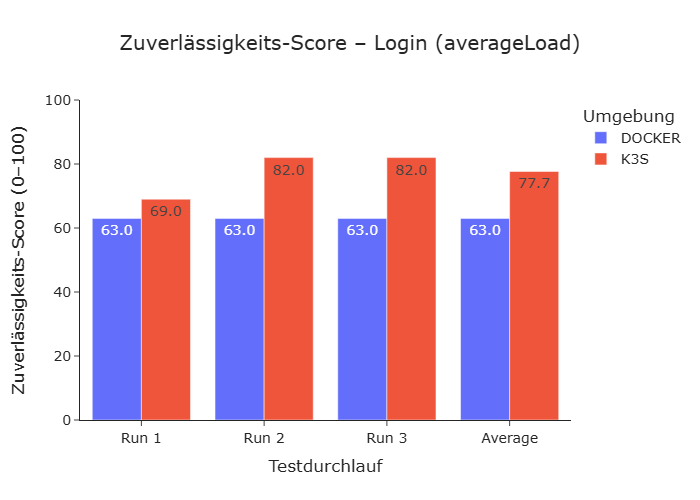
\includegraphics[width=0.8\textwidth]{bilder/tests/reliability_score_login_averageLoad.png}
\caption{Reliability Score für das Login-Szenario unter Average Load}
\label{fig:login_reliability_score}
\end{figure}

Vergleichen wir nun die durchschnittliche Zuverlässigkeit der Score-Werte jedes Tests des Login-Szenarios, die in der Tabelle \ref{tab:scenario_score_matrix_login} zu sehen ist, so zeigt sich, dass die k3s-Umgebung bei jedem Test die bessere Zuverlässigkeit erreicht, bis auf den Smoke-Test bei dem beide die Maximalpunktzahl erreichen konnten.
Bis auf den Spike-Test bleiben beide Umgebungen nah beieinander.

\begin{table}[htbp]
\centering
\caption{Durchschnittlicher Reliability Score pro Testtyp für das Szenario Login}
\label{tab:scenario_score_matrix_login}

\begin{tabular}{lccccc}
\toprule
\textbf{Environment} & \textbf{Smoke} & \textbf{Average Load} & \textbf{Stress} & \textbf{Spike} & \textbf{Breaking Point} \\
\midrule
Docker & 100.00 & 63.00 & 59.67 & 38.00 & 53.00 \\
K3s    & 100.00 & 77.67 & 65.00 & 60.00 & 65.00 \\
\bottomrule
\end{tabular}

\end{table}

\FloatBarrier
\subsubsection{Vorlesungen}
Wie in Abbildung \ref{fig:vorlesungen_reliability_score} zu sehen ist, hat bei den Vorlesungen unter Average Load kein Testdurchlauf einen Score über 50 von 100 Punkten erreicht.
Die k3s-Umgebung hat dabei wieder einen höheren Score als die Docker-Compose-Umgebung erhalten.
In den in Tabelle \ref{tab:vorlesungen_average_load_metrics} aufgeführten Messwerten ist besonders interessant, dass beide Umgebungen eine hohe Fehlerrate für eine Webanwendung aufweisen.
Dabei hat die k3s-Umgebung fast doppelt so viele Fehler wie die Docker-Compose-Umgebung.
Trotz der niedrigeren Fehlerrate hat die Anwendung in der Docker-Compose-Umgebung einen höheren CPU- und RAM-Verbrauch als die k3s-Umgebung.
\begin{table}[htbp]
\centering
\caption{Vergleich der Durchschnittswerte aller Test zur bestimmung der Zuverlässigkeit für das Vorlesungen-Szenario unter Average Load}
\label{tab:vorlesungen_average_load_metrics}

\begin{tabular}{lrr}
\toprule
\textbf{Metrik} & \textbf{Docker} & \textbf{K3s} \\
\midrule
Error Rate [\%]        & 2.38 & 4.65 \\
CPU Max [\%]           & 99.57 & 44.18 \\
Memory Max [\%]        & 74.66 & 23.58 \\
Node CPU Max [\%]      & 99.98 & 109.63 \\
Node Memory Max [\%]   & 81.25 & 81.02 \\
Restarts               & 0.00 & 0.00 \\
\bottomrule
\end{tabular}

\end{table}

\begin{figure}[htbp]
\centering
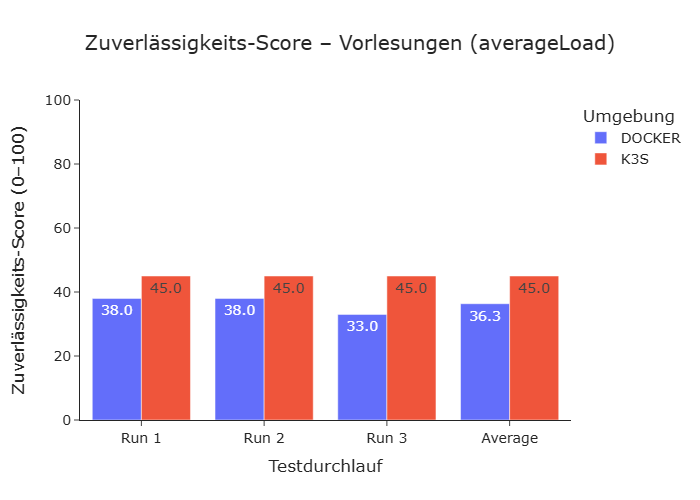
\includegraphics[width=0.8\textwidth]{bilder/tests/reliability_score_vorlesungen_averageLoad.png}
\caption{Reliability Score für das Vorlesungen-Szenario unter Average Load}
\label{fig:vorlesungen_reliability_score}
\end{figure}

Ein Vergleich der durchschnittlichen Zuverlässigkeitsscores jeder Testmethode in dem Szenario „Vorlesungen“, wie in Tabelle \ref{tab:scenario_score_matrix_vorlesungen} dargestellt, zeigt, dass die Docker-Compose-Umgebung in den meisten Testmethoden einen höheren Score erreichen konnte.
Nur beim „Average Load” konnte die „k3s”-Umgebung einen höheren Score als die „Docker Compose”-Umgebung erzielen. 
Bei „Smoke” haben beide Umgebungen wieder den gleichen Score erzielt.
Die Abstände zwischen den Umgebungen sind jeweils nicht allzu groß.

\begin{table}[htbp]
\centering
\caption{Durchschnittlicher Reliability Score pro Testtyp für das Szenario Vorlesungen}
\label{tab:scenario_score_matrix_vorlesungen}

\begin{tabular}{lccccc}
\toprule
\textbf{Environment} & \textbf{Smoke} & \textbf{Average Load} & \textbf{Stress} & \textbf{Spike} & \textbf{Breaking Point} \\
\midrule
Docker & 75.00 & 36.33 & 38.00 & 38.00 & 38.00 \\
K3s    & 75.00 & 45.00 & 31.67 & 25.00 & 25.00 \\
\bottomrule
\end{tabular}

\end{table}

\FloatBarrier
\subsubsection{Klausur}
Wie in Abbildung \ref{fig:klausur_reliability_score} zu sehen ist, blieb der Score bei den Klausuren unter Average Load bei jedem Testdurchlauf unter 20 von 100 Punkten.
Im zweiten Testdurchlauf gab es einen Ausschlag der k3s-Umgebung, in der ein Score von 0 Punkten erreicht wurde.
In den übrigen Testdurchläufen konnte die k3s-Umgebung einen besseren Score erzielen, blieb aber jedes Mal unter dem Score der Docker-Compose-Umgebung.
Dabei kann in Tabelle \ref{tab:klausur_average_load_metrics} erneut eine hohe Fehlerrate festgestellt werden, wobei diese in der Docker-Compose-Umgebung mehr als die Hälfte kleiner ist als in der k3s-Umgebung.
Die Anwendung in der Docker-Compose-Umgebung verbraucht aber wieder deutlich mehr CPU als in der k3s-Umgebung.
Auffällig ist auch, dass die k3s-Umgebung achtmal Pods neustarten musste.

\begin{table}[htbp]
\centering
\caption{Vergleich der Durchschnittswerte aller Test zur bestimmung der Zuverlässigkeit für das Klausur-Szenario unter Average Load}
\label{tab:klausur_average_load_metrics}

\begin{tabular}{lrr}
\toprule
\textbf{Metrik} & \textbf{Docker} & \textbf{K3s} \\
\midrule
Error Rate [\%]        & 5.43 & 12.05 \\
CPU Max [\%]           & 99.64 & 27.91 \\
Memory Max [\%]        & 63.12 & 19.80 \\
Node CPU Max [\%]      & 99.67 & 101.98 \\
Node Memory Max [\%]   & 66.95 & 78.60 \\
Restarts               & 0.00 & 8.00 \\
\bottomrule
\end{tabular}

\end{table}

\begin{figure}[htbp]
\centering
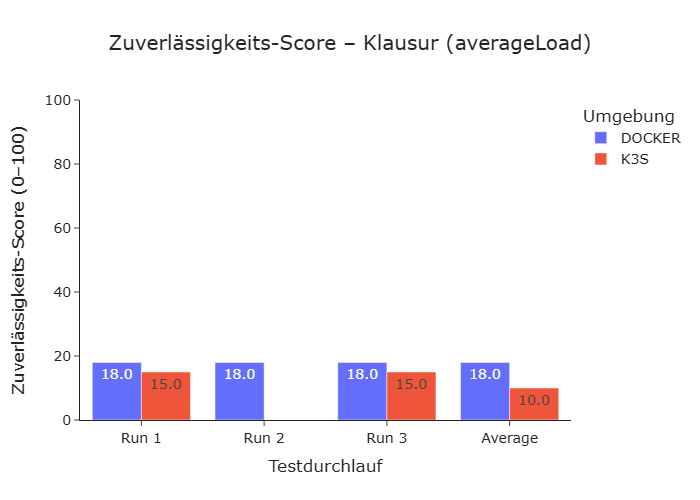
\includegraphics[width=0.8\textwidth]{bilder/tests/reliability_score_klausur_averageLoad.png}
\caption{Reliability Score für das Klausur-Szenario unter Average Load}
\label{fig:klausur_reliability_score}
\end{figure}

Beim Vergleich der durchschnittlichen Zuverlässigkeitswerte jeder Testmethode im Szenario „Klausur“, die in der Tabelle \ref{tab:scenario_score_matrix_klausur} zu sehen ist, fällt auf, dass die Docker-Compose-Umgebung wieder fast immer einen höheren Score als die k3s-Umgebung erzielt hat, bis auf den Spike-Test.
Dennoch bleibt festzuhalten, dass sich die Umgebungen nicht zu stark unterscheiden.
\begin{table}[htbp]
\centering
\caption{Durchschnittlicher Reliability Score pro Testtyp für das Szenario Klausur}
\label{tab:scenario_score_matrix_klausur}

\begin{tabular}{lccccc}
\toprule
\textbf{Environment} & \textbf{Smoke} & \textbf{Average Load} & \textbf{Stress} & \textbf{Spike} & \textbf{Breaking Point} \\
\midrule
Docker & 55.00 & 18.00 & 18.00 & 18.00 & 18.00 \\
K3s    & 41.33 & 10.00 & 17.00 & 23.00 & 6.67 \\
\bottomrule
\end{tabular}

\end{table}
\FloatBarrier
\subsection{Chaos-Test}
Bei den Chaos-Tests werden die Ergebnisse der Szenarien auf der Haupt-API vorgestellt.
Dabei werden die wichtigsten Testdaten zur Bestimmung der Zuverlässigkeit jedes Testdurchlaufs präsentiert.
Die angezeigten Werte sind eine Aggregation aller Testdurchläufe.
Einerseits wird gezeigt, wie durchschnittlich verfügbar die Anwendung während des Tests war.
Die durchschnittliche Fehlerrate wird ebenfalls bewertet.
Dazu kommt, wie lange das System im Durchschnitt gebraucht hat, um die Services wiederherzustellen, und bei wie vielen Testdurchläufe die Umgebungen innerhalb eines Test dies hinbekommen haben.

Zum Schluss jedes Szenarios wird die Auswertung jedes Testdurchlaufs angezeigt und wie der durchschnittliche Score der Testdurchläufe war.

\subsubsection{Teilausfall bei der Haupt-API}

Bei einem Teilausfall der Haupt-API hat die Docker-Compose-Umgebung es bei keinem Testdurchlauf geschafft, den Service innerhalb des Testfensters selbst wiederherzustellen, wie in der Tabelle \ref{tab:chaos_api_instance_down} zu sehen ist.
Dadurch hat Docker keinen der Tests bestanden, weshalb der Zuverlässigkeits-Score der Docker-Compose-Umgebung bei jeder Testumgebung eine 0 beträgt, wie in Abbildung \ref{fig:chaos_api_instance_down} zu sehen ist. 
Die k3s-Umgebung hat dagegen jeweils einen Score von 60 Punkten oder mehr erzielt.
Zur Wiederherstellung des Services hat k3s im Durchschnitt weniger als eine Sekunde gebraucht. Da die Docker-Compose-Umgebung den Service nicht von selbst wiederherstellen konnte, wurde keine Zeit eingetragen, da diese nur die Länge vom Chaos-Anfang bis Testende betragen würde. 
\begin{table}[htbp]
\centering
\caption{Vergleich der Chaos-Test-Metriken bei Teilausfall der Haupt-API}
\label{tab:chaos_api_instance_down}

\begin{tabular}{lrr}
\toprule
\textbf{Metrik} & \textbf{Docker} & \textbf{K3s} \\
\midrule
Error Rate [\%]         & 98.96 & 3.11 \\
Availability [\%]       & 1.04 & 96.89 \\
Recovery Time [s]      & - & 0.44 \\
Recovered [Anzahl]      & 0 & 3 \\
\bottomrule
\end{tabular}

\end{table}

\begin{figure}[htbp]
\centering
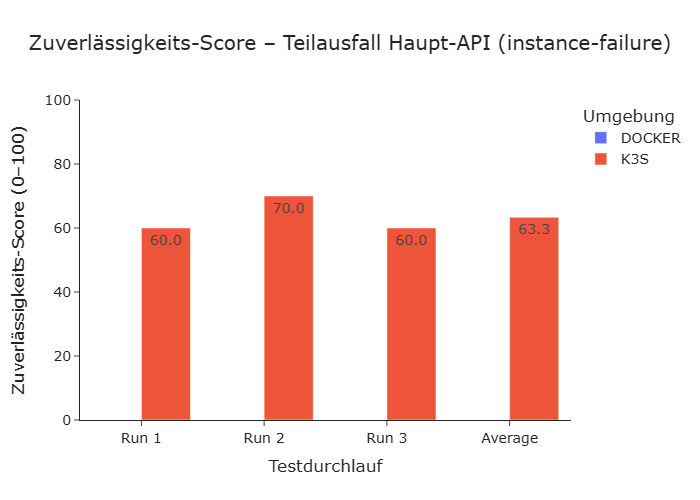
\includegraphics[width=0.8\textwidth]{bilder/tests/reliability_score_api-instance-down_instance-failure.png}
\caption{Zuverlässigkeit Score bei Teilausfall der Haupt-API}
\label{fig:chaos_api_instance_down}
\end{figure}
\FloatBarrier
\subsubsection{Komplettausfall der Haupt-API}
Bei einem Komplettausfall der Haupt-API hat die Docker-Compose-Umgebung es wieder nicht hinbekommen, den Service von selbst wiederherzustellen. Deshalb hat die Docker-Compose-Umgebung in der Abbildung \ref{fig:chaos_api_outage} in jedem Testdurchlauf 0 von 100 Punkten.
Der Score von Kubernetes beträgt bei jedem Testdurchlauf 35 von 100.
In der Tabelle \ref{tab:chaos_api_outage} ist zu sehen, dass die k3s-Umgebung eine niedrige Verfügbarkeit und eine höhere Fehlerrate hatte.
Die k3s-Umgebung hat im Durchschnitt unter zwanzig Sekunden benötigt, um den Service wiederherzustellen. 
Da die Docker-Compose-Umgebung es nicht innerhalb des Testfensters geschafft hat, den Service wiederherzustellen, wurde keine Zeit eingetragen, da diese nur die Zeit vom Chaos-Anfang bis Testende darstellen würde.

\begin{table}[htbp]
\centering
\caption{Vergleich der Chaos-Test-Metriken bei Komplettausfall der Haupt-API}
\label{tab:chaos_api_outage}

\begin{tabular}{lrr}
\toprule
\textbf{Metrik} & \textbf{Docker} & \textbf{K3s} \\
\midrule
Error Rate [\%]                    & 98.97 & 5.63 \\
Availability [\%]                & 1.03 & 94.37 \\
Recovery Time [s]                 & - & 17.29 \\
Recovered [Anzahl]                 & 0 & 3 \\
\bottomrule
\end{tabular}

\end{table}

\begin{figure}[htbp]
\centering
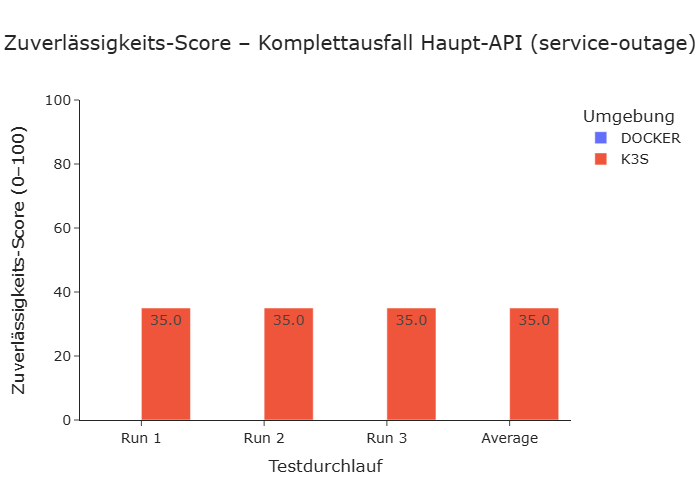
\includegraphics[width=0.8\textwidth]{bilder/tests/reliability_score_api-outage_service-outage.png}
\caption{Zuverlässigkeit Score bei Komplettausfall der Haupt-API}
\label{fig:chaos_api_outage}
\end{figure}
\FloatBarrier
\subsubsection{Update der Haupt-API}
Bei einem Update der Haupt-API hat die Docker-Compose-Umgebung in jedem Testlauf den Score 35 von 100 erzielt, während die k3s-Umgebung mit dem Score 70 von 100 in jedem Testlauf das Doppelte erreicht hat.
In der Tabelle \ref{tab:chaos_api_update} benötigte die Docker-Compose-Umgebung im Durchschnitt 21,38 Sekunden, um den Service wiederherzustellen, während es bei der k3s-Umgebung zu keinem Ausfall kam.
\begin{table}[htbp]
\centering
\caption{Vergleich der Chaos-Test-Metriken bei Update der Haupt-API}
\label{tab:chaos_api_update}

\begin{tabular}{lrr}
\toprule
\textbf{Metrik} & \textbf{Docker} & \textbf{K3s} \\
\midrule
Error Rate [\%]                    & 7.76 & 3.12 \\
Availability [\%]                & 92.24 & 96.88 \\
Recovery Time [s]       & 21.38 & 0.00 \\
Recovered [Anzahl]  & 3 & 3 \\
\bottomrule
\end{tabular}

\end{table}

\begin{figure}[htbp]
\centering
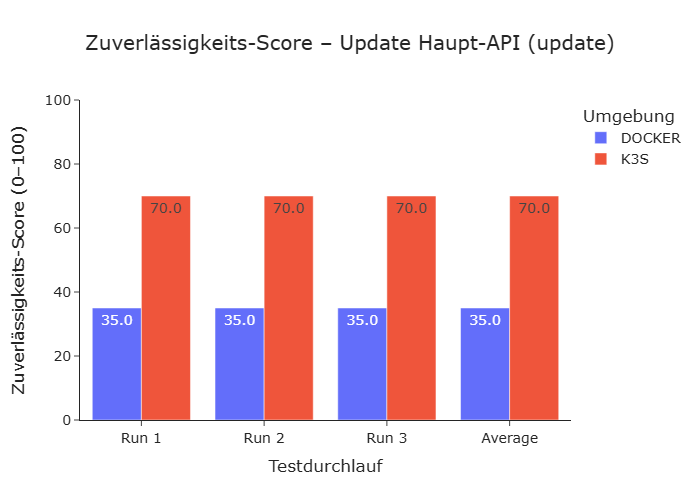
\includegraphics[width=0.8\textwidth]{bilder/tests/reliability_score_api-update_update.png}
\caption{Zuverlässigkeit Score bei Update der Haupt-API}
\label{fig:chaos_api_update}
\end{figure}
\FloatBarrier
\section{Diskussion der Ergebnisse}
Nachdem die Ergebnisse der Tests vorgestellt wurden, werden im Folgenden die Ursachen dieser Testergebnisse erörtert.
Eine der ersten Dinge, die bei den Loadtests auffallen, ist, dass die Scores der Docker-Compose- und der k3s-Umgebung üblicherweise relativ nah beieinander liegen.
Das liegt daran, dass Codetask aktuell ein eher kleines System mit einer noch überschaubaren Nutzeranzahl ist, wodurch ein Lastverbrauch entsteht, mit dem Docker Compose mithalten kann.

Das führt direkt zum nächsten Punkt, der in den Testergebnissen auffällt. 
Die Docker-Compose-Umgebung schneidet in den meisten Loadtests besser ab als die k3s-Umgebung, obwohl die k3s-Umgebung in Bezug auf die Zuverlässigkeit im Vorteil sein sollte.
Das liegt daran, dass die Ergebnisse der Loadtests von der Performance einer Anwendung beeinflusst werden.
Kubernetes selbst ist kein Performance-Optimierer, sondern soll eine Anwendung stabil halten. Dadurch ist eine höhere Zuverlässigkeit oft nicht direkt sichtbar.
In den Testwerten des Vorlesungs- und Klausur-Szenarios fällt auf, dass k3s eine höhere Fehlerrate als die Docker-Compose-Umgebung hat.
In Tabelle \ref{tab:klausur_average_load_metrics} sind sogar Restarts von Pods bei Kubernetes vermerkt, während bei Docker Compose kein Restart aufgeführt ist.
Dadurch wirkt die k3s-Umgebung auf den ersten Blick unzuverlässiger. Dabei handelt es sich jedoch nicht um ein Problem mit der Zuverlässigkeit, sondern um ein Performanceproblem, genauer gesagt um den massiven Ressourcenverbrauch der Check-API.
Zwar ist es logisch, dass die Check-API durch den von ihr betriebenen Compiler mehr Ressourcen benötigt, für einen erhöhten Nutzen der Check-API werden jedoch fast vier CPU-Kerne benötigt.
Dies ist das Maximum, das die VMs aus der Docker-Compose- und der k3s-Umgebung haben. Deshalb versucht die Check-API, alle Ressourcen für sich zu beanspruchen.
In der Docker-Compose-Umgebung fällt dies jedoch nicht auf, da RAM und CPU dort nach dem Best-Effort-Prinzip verteilt werden und ein Service somit mehr Ressourcen beanspruchen kann, als fair ist.
Bei Kubernetes hat allerdings jeder Pod einen Request, also einen Mindestbedarf an Ressourcen, aber auch ein Limit für den CPU- und RAM-Verbrauch. 
Daher können die Services die Ressourcen nicht frei nutzen.
Aufgrund dieser Limitierung kann die Check-API nicht mehr auf die benötigten Ressourcen zugreifen. Dadurch wird sie langsamer und muss häufiger neu gestartet werden, je mehr sie genutzt wird.
Dies kann durch mehrere Ergebnisse bewiesen werden. Erstens haben beide Umgebungen im Login-Szenario, in dem die Check-API nicht genutzt wird, ein besseres Scoring.
Zweitens ist das Scoring der k3s-Umgebung in Tests, bei denen mehr virtuelle User verwendet werden, schlechter, da die Check-API häufiger genutzt werden muss. Die Docker-Compose-Umgebung kann dies besser verwalten.
Dabei versteckt die Docker-Compose-Umgebung die Performance-Probleme eher, während die k3s-Umgebung diese messbarer und sichtbarer macht.
Dadurch wird die Anwendung instabiler, da die Check-API die Ressourcen in der Docker-Compose-Umgebung für sich beansprucht. In der k3s-Umgebung läuft die Check-API zwar schlechter, kann aber die restlichen Services nicht beeinflussen.
Dies spricht eher für eine bessere Zuverlässigkeit der k3s-Umgebung, da die Anwendung insgesamt stabiler ist und sich die einzelnen Services weniger stark beeinflussen können.

Die Testergebnisse zeigen, dass die Unterschiede zwischen der Docker-Compose- und der k3s-Umgebung durch die Chaos-Tests deutlicher sichtbar sind als durch die Loadtests.
Das deutet darauf hin, dass die k3s-Umgebung toleranter gegenüber Ausfällen ist als die Docker-Compose-Umgebung, da bereits ein Teilausfall eines Dienstes bedeutet, dass der Dienst komplett ausgefallen ist, während die k3s-Umgebung noch erreichbar ist.
Die Wiederherstellungszeit in der Tabelle \ref{tab:chaos_api_instance_down} bei k3s ist wahrscheinlich eher auf den Timer der Testumgebung als auf eine Downtime des Services zurückzuführen.
Dieses Verhalten wurde dadurch verschärft, dass auch aus den Ergebnissen zu entnehmen ist, dass die Docker-Compose-Umgebung trotz festgelegter Restart-Regeln nicht in der Lage war, sich selbst wiederherzustellen.
Das passierte dadurch, dass der Container bei einem Absturz in einen Restart-Loop gerät.
Das wird durch einen persistenten RUNNING\_PID-Zustand verursacht, weswegen der Container beim Hochfahren glaubt, dass dieser Service schon betrieben wird. Dadurch entscheidet er, dass es diesen Service nicht doppelt geben darf, beendet sich wieder und die Restart-Policy greift erneut.
Dieser Fehler tritt anscheinend nicht bei einem kontrollierten Herunterfahren des Containers auf, was durch die Ergebnisse des Update-Tests gezeigt wird. 

Dort wird durch das Webhook-Skript die gesamte Docker-Compose-Umgebung heruntergefahren und anschließend neu gestartet. Durch diese Deployment-Verwaltung hat die Docker-Compose-Umgebung auch eine Downtime beim Deployment.
Durch dieses Webhook-Deployment fallen auch direkt alle Services aus, selbst wenn diese eigentlich kein Update haben. Dadurch könnte ein Update der AI-API auch die Haupt-API kurzzeitig down bringen.
Bei kleineren Deployments, bei denen nichts Neues erstellt wird, ist das eher eine geringe Auswirkung, wie in der Tabelle \ref{tab:chaos_api_update} zu sehen ist. Bei größeren Deployments kann das aber auch länger dauern.
Zusätzlich ist beim Erstellen der Update-Tests ein Bug aufgefallen, wodurch das Webhook-Skript, das zum Deployment genutzt wird, die Anwendungen von der VM entfernen kann.
Das passiert, weil das Skript nach dem Klonen des Projekts auf die VM den alten Projektstand blind löscht, auch wenn beim Klonen ein Fehler aufgetreten ist, wodurch der neue Projektzustand nicht auf der VM vorhanden ist.
Die Volumes sind davon nicht betroffen, aber alles andere, das sich im Ordner „teamprojekt” befindet, darunter das Docker Compose, das Webhook-Skript selbst und auch die TLS-Zertifikate.

Dies ist jedoch eher ein Problem der Deployment-Verwaltung durch den Webhook als durch Docker Compose selbst. Aber auch wenn die Services einzeln aktualisiert werden, gäbe es eine Downtime.
In der k3s-Umgebung wird das Rolling Update angewendet, wodurch, wie in Tabelle \ref{tab:chaos_api_update} zu sehen ist, eine Zero-Downtime erreicht wird. Das passiert, da die Pods nach und nach ersetzt werden, anstatt dass der gesamte Service heruntergefahren wird.
Durch die Deployment-Verwaltung mit FluxCD übernimmt die k3s-Umgebung das Deployment selbst, wodurch dieser Fehler mit dem Webhook nicht auftreten kann.

